\chapter{电与磁作为同一个相对论性场}

我们已经研究了给定的电磁场如何使带电粒子运动。问题尚未完成的一半是场本身：电场和磁场如何演化，以及电荷和电流如何作为它们的源。麦克斯韦方程组回答了这些问题。然而，在写出它们之前，值得重新回顾那个使它们的相对论性结构不可避免的物理谜题。

这是有意从形式化体系退后一步。作用量原理将会回来，但不是现在。从别处开始的目的，是要在从作用量导出动力学之前，先看清为什么电场和磁场必须是同一个对象的组成部分。

\section{爱因斯坦第一段中的谜题}

在访问比利时期间，一场关于早期索尔维会议的讨论引回到了爱因斯坦1905年的论文\emph{《论动体的电动力学》}。它的第一段以非凡的简洁陈述了动机。同一个电磁现象在两个惯性系中得到两种表面上不同的解释。一个观察者称该效应为磁的；另一个称它为电的。所观察到的运动一致，因此这两种描述不可能代表两块不同的物理。

这篇论文现在已可按本课程所发展的水平来理解。即使不逐一推演每个计算，开篇段落也值得一读，因为它在引入答案之前提出了正确的问题：电的描述和磁的描述如何能够改变，而物理事件却不改变？

\subsection{一个电荷、一块磁体，以及两种描述}

取一个指向\(y\)方向的磁场，以及一个沿\(x\)轴运动的电荷。在实验室系中电场为零，因此力是磁力：
\begin{equation}
\mathbf F=q\,\mathbf v\times\mathbf B.
\end{equation}
它指向剩下的横向方向。课堂上快速画出的坐标轴并不意在确定每一个右手定则的符号；重要的事实是力同时垂直于\(\mathbf v\)和\(\mathbf B\)，并且改变电荷的符号会反转力的方向。

\begin{classroomqa}
\audiencequestion{在图中力指向上还是向下？}
\lecturerresponse{这取决于电荷的符号。一旦坐标轴的方向和\(q\)的符号确定，右手定则就确定了方向。就目前的论证而言，只有横向力的存在才是重要的。\lecturetimestamp{00:07:13}}
\end{classroomqa}

爱因斯坦描述的是导线而非孤立粒子。原子提供了一个近似固定的点阵，而可移动的载流子在其中运动。在二十世纪初，导线中的电流也比一个自由带电粒子的轨迹容易观察得多。这一区别在这里无关紧要：磁场中运动的载流子感受到相同的洛伦兹力。

\begin{figure}[H]
\centering
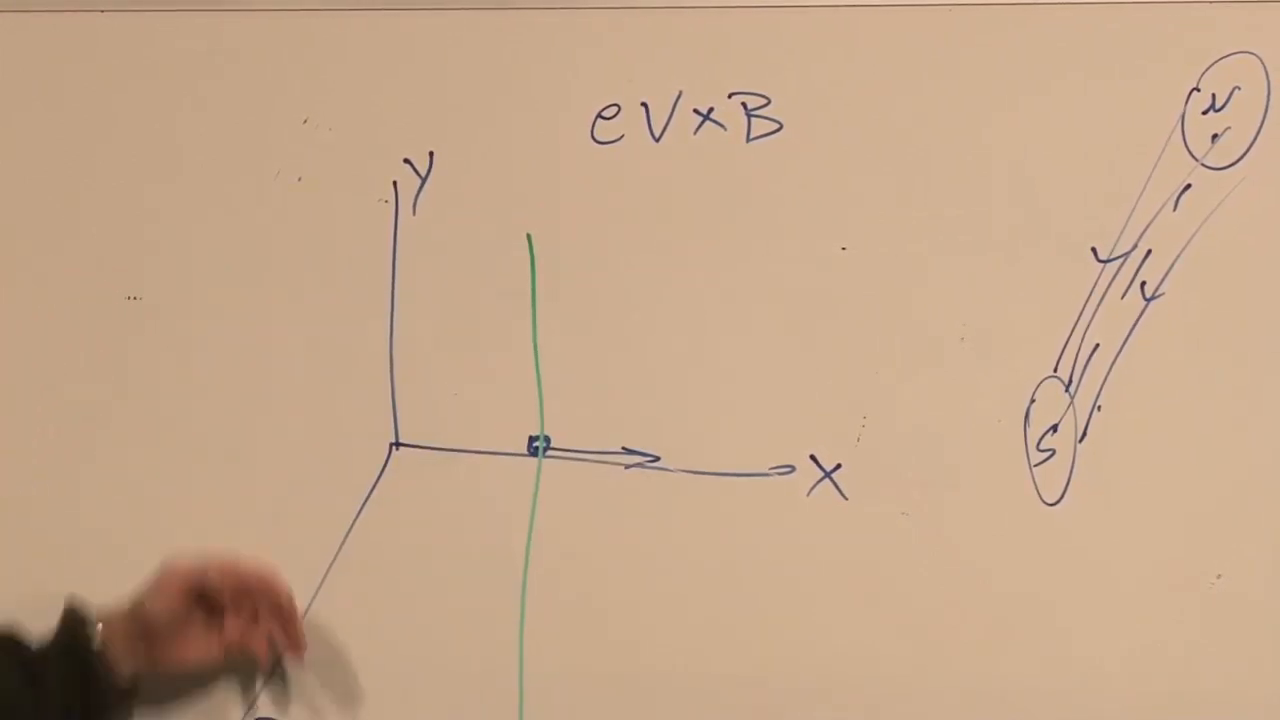
\includegraphics[width=\linewidth]{lecture_08_figure_01.png}
\caption{用于重述爱因斯坦电动力学谜题的运动电荷、横向磁场和磁体几何。}
\par\smallskip
\textit{课堂时间戳：00:07:00。}
\end{figure}

现在保持导线或检验电荷固定，改为移动磁体。变化的磁场位形产生一个电动势，用局部的语言说就是一个电场。该电场沿相同的横向方向推动静止电荷。因此这两种描述是
\begin{align}
\text{moving charge, fixed magnet:}\quad&
q\,\mathbf v\times\mathbf B,
\\
\text{fixed charge, moving magnet:}\quad&
q\,\mathbf E'.
\end{align}
相对运动是相同的。因此，相对论理论必须解释一个在一个系中纯为磁性的场如何在另一个系中获得电的分量。

电和磁不是彼此分离的实体。它们是同一个相对论性场的依赖于系的组成部分。爱因斯坦当时还没有现代的场张量记号，他在这一段中也没有把所需的系变换称为洛伦兹变换。尽管如此，变换的问题已经完整地存在了。

\section{电磁场张量}

能够把电的数据和磁的数据一起携带的对象是反对称张量
\begin{equation}
F_{\mu\nu}
=
\partial_\mu A_\nu-\partial_\nu A_\mu.
\label{eq:field-tensor-definition}
\end{equation}
希腊指标取遍\(0,1,2,3\)，其中\(x^0=t\)；拉丁指标取遍三个空间值。反对称性
\begin{equation}
F_{\mu\nu}=-F_{\nu\mu},
\end{equation}
使对角元为零，并留下六个独立分量。这六个分量恰好就是\(\mathbf E\)的三个分量和\(\mathbf B\)的三个分量。

在主要为正的度规
\begin{equation}
\eta_{\mu\nu}=\operatorname{diag}(-1,1,1,1),
\end{equation}
以及从上一讲带电粒子作用量继承来的约定下，定义
\begin{align}
E_m&=F_{0m}
=\partial_0A_m-\partial_mA_0,
\label{eq:e-from-a}
\\
B_i&=(\boldsymbol\nabla\times\mathbf A)_i.
\label{eq:b-from-a}
\end{align}
讲义在写第一行时更正了一个空间指标。干净的关系式就是上面这个：自由的空间指标在两边必须一致。

\begin{figure}[H]
\centering
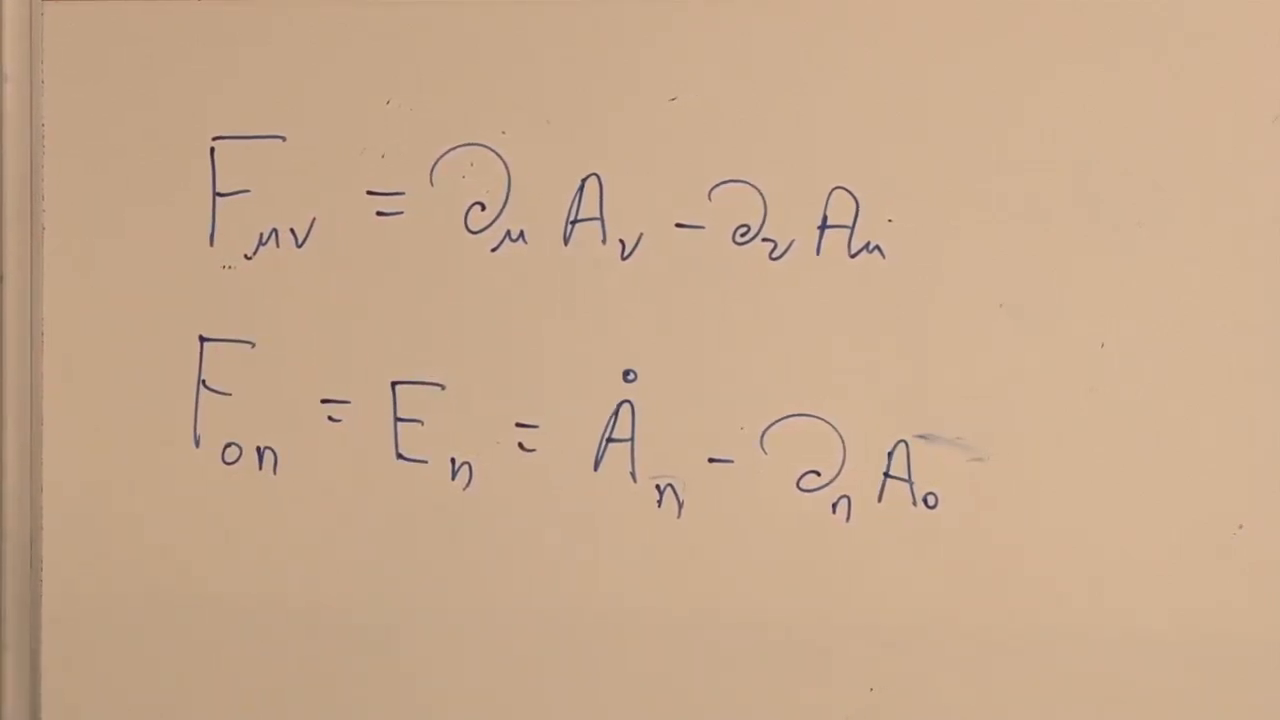
\includegraphics[width=\linewidth]{lecture_08_figure_02.png}
\caption{场张量的定义，以及与电场相对应的混合时间--空间分量。}
\par\smallskip
\textit{讲义帧：00:13:15。}
\end{figure}

磁感应关系是同一空间部分定义。例如，
\begin{equation}
B_x
=
\partial_yA_z-\partial_zA_y
=
F_{yz},
\end{equation}
其余两个分量由循环置换得到。

\begin{figure}[H]
\centering
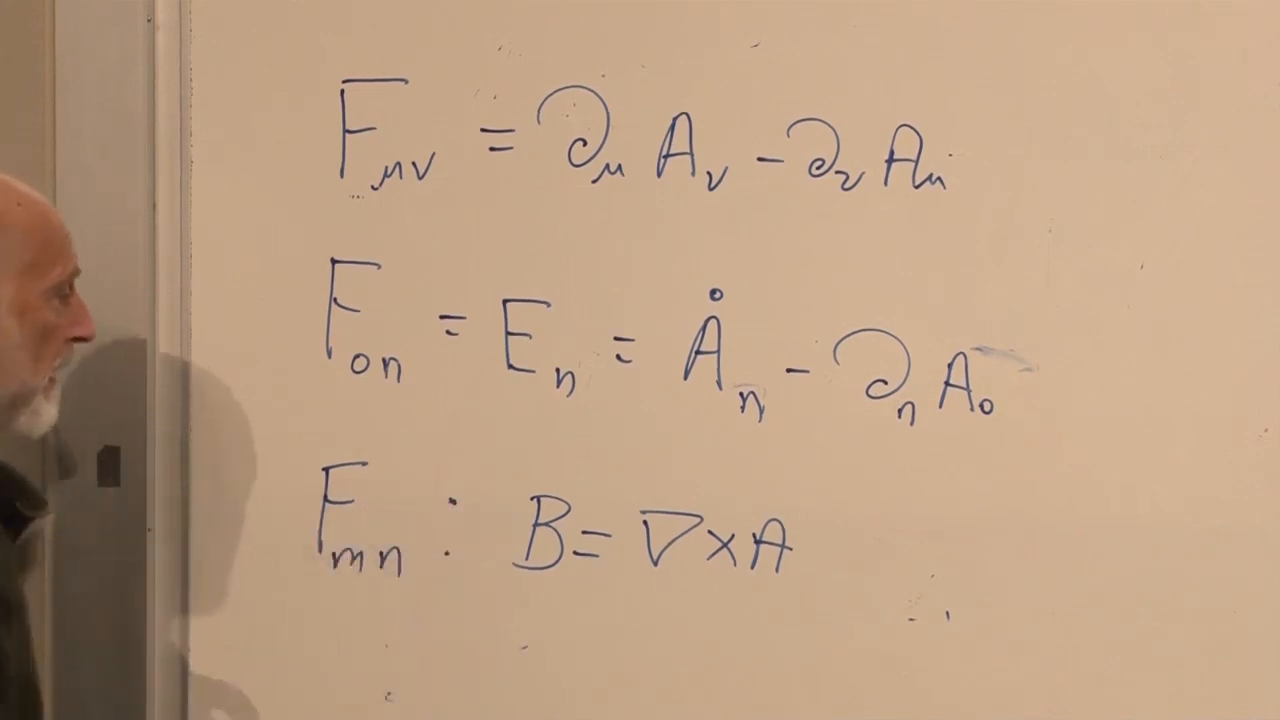
\includegraphics[width=\linewidth]{lecture_08_figure_03.png}
\caption{电场和磁场旋度的矢量势公式已列在黑板上。}
\par\smallskip
\textit{讲义帧：00:14:00。}
\end{figure}

\subsection{分量阵列}

令第一个张量指标标记行，第二个指标标记列，按\(0,x,y,z\)排序。于是
\begin{equation}
F_{\mu\nu}
=
\begin{pmatrix}
0&E_x&E_y&E_z\\
-E_x&0&B_z&-B_y\\
-E_y&-B_z&0&B_x\\
-E_z&B_y&-B_x&0
\end{pmatrix}.
\label{eq:f-lower-matrix}
\end{equation}
混合时间--空间边缘包含\(\mathbf E\)；空间\(3\times3\)块包含\(\mathbf B\)。下三角不是新信息，因为它是上三角的负反射。

\begin{figure}[H]
\centering
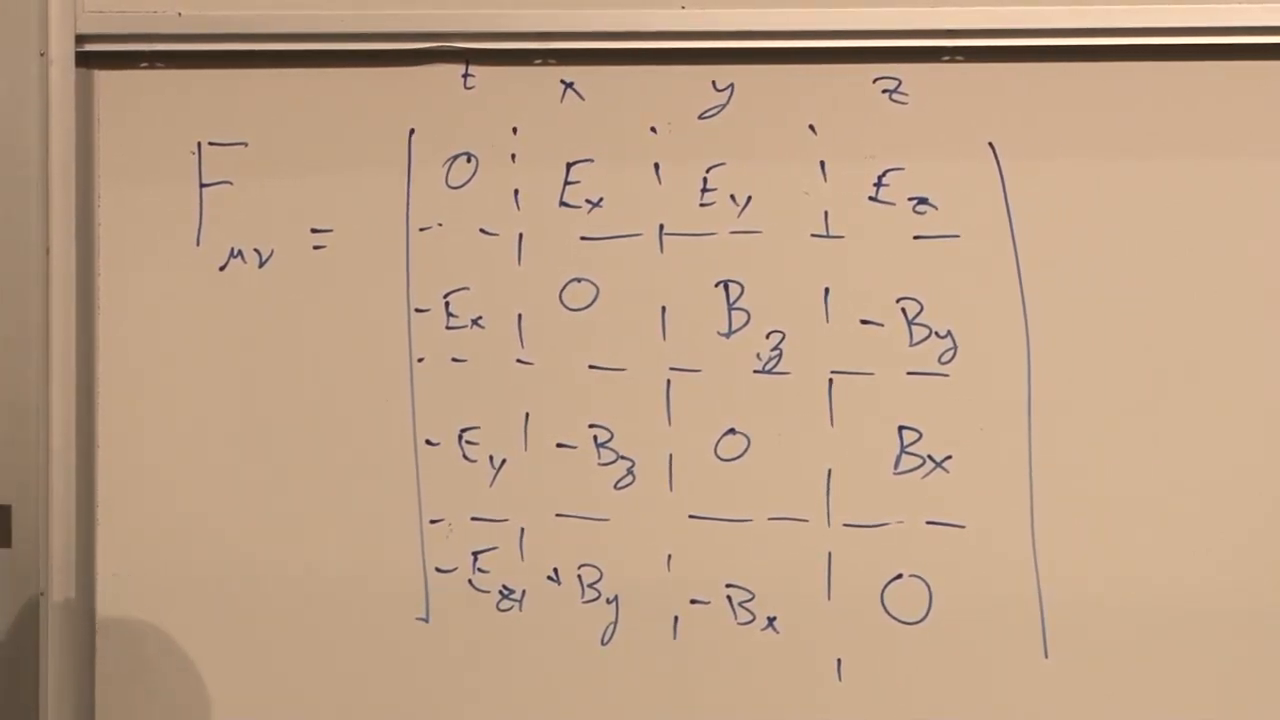
\includegraphics[width=\linewidth]{lecture_08_figure_04.png}
\caption{完成的下指标电磁张量，其电边缘和磁空间块。}
\par\smallskip
\textit{讲义帧：00:17:15。}
\end{figure}

提升两个指标会改变每个电分量的符号，而磁分量保持不变：
\begin{equation}
F^{\mu\nu}
=
\begin{pmatrix}
0&-E_x&-E_y&-E_z\\
E_x&0&B_z&-B_y\\
E_y&-B_z&0&B_x\\
E_z&B_y&-B_x&0
\end{pmatrix}.
\label{eq:f-upper-matrix}
\end{equation}
电分量带有一个时间指标，因此获得一个负号。磁分量带有两个空间指标，因此不获得负号。

\begin{classroomqa}
\audiencequestion{我是否正确理解矩阵，即磁分量没有时间指标？}
\lecturerresponse{是的。它们占据纯空间块。电分量正是沿第一行和第一列的混合时间--空间项。\lecturetimestamp{00:18:55}}
\end{classroomqa}

\section{提升纯磁场}

考虑沿\(x\)的助推，其中\(c=1\)：
\begin{align}
t'&=\gamma(t-vx),
&
x'&=\gamma(x-vt),
&
y'&=y,
&
z'&=z,
\end{align}
其中
\begin{equation}
\gamma=\frac{1}{\sqrt{1-v^2}}.
\end{equation}
以矩阵形式，
\begin{equation}
x'^\mu
=
\Lambda^\mu{}_\nu x^\nu,
\qquad
\Lambda^\mu{}_\nu
=
\begin{pmatrix}
\gamma&-\gamma v&0&0\\
-\gamma v&\gamma&0&0\\
0&0&1&0\\
0&0&0&1
\end{pmatrix}.
\label{eq:x-boost}
\end{equation}

\begin{classroomqa}
\audiencequestion{助推矩阵中是否缺少一个负号？}
\lecturerresponse{是的。非对角时间--空间项带有\(t'=\gamma(t-vx)\)和\(x'=\gamma(x-vt)\)所要求的负号。在使用场变换之前已进行修正。\lecturetimestamp{00:23:50}}
\end{classroomqa}

\begin{figure}[H]
\centering
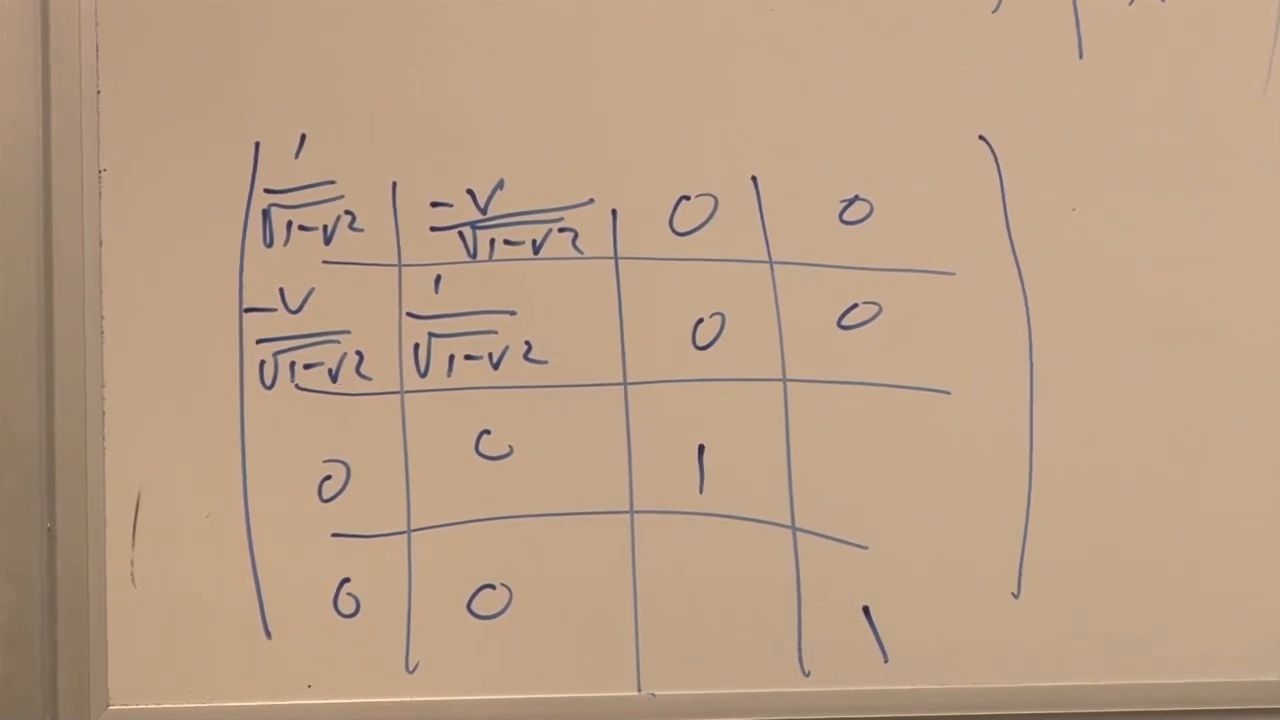
\includegraphics[width=\linewidth]{lecture_08_figure_05.png}
\caption{沿\(x\)轴运动的修正洛伦兹助推矩阵。}
\par\smallskip
\textit{讲义帧：00:24:00。}
\end{figure}

每个上张量指标都像上矢量指标一样变换。因此
\begin{equation}
F'^{\mu\nu}
=
\Lambda^\mu{}_\sigma
\Lambda^\nu{}_\tau
F^{\sigma\tau}.
\label{eq:f-boost-law}
\end{equation}
重复的\(\sigma\)和\(\tau\)是哑指标。对于具有更多指标的张量，每个指标都会出现一个变换矩阵。

\begin{figure}[H]
\centering
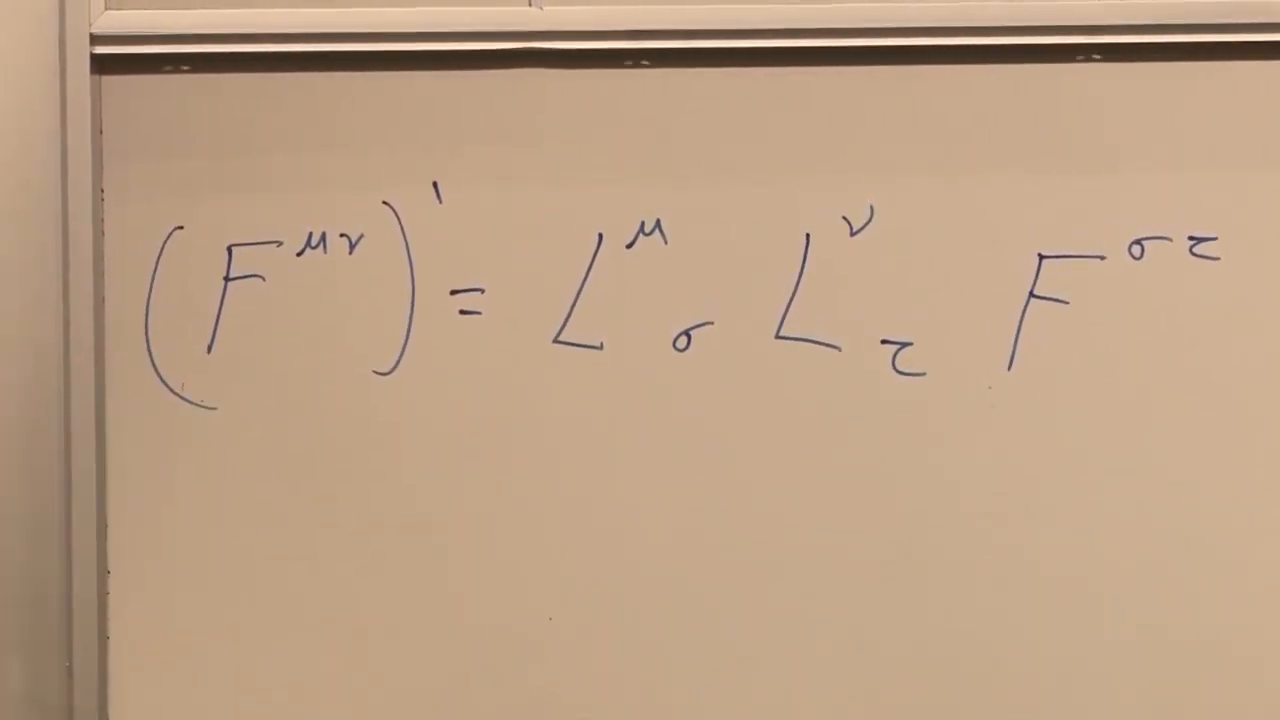
\includegraphics[width=\linewidth]{lecture_08_figure_06.png}
\caption{二阶洛伦兹变换定律，每个场张量指标对应一个助推矩阵。}
\par\smallskip
\textit{讲义帧：00:26:40。}
\end{figure}

\subsection{变为电场的分量}

假设未加撇的参考系仅包含磁场\(B_y\)。在方程~\eqref{eq:f-upper-matrix}的约定下，相关的独立分量为
\begin{equation}
F^{xz}=-B_y.
\end{equation}
我们寻求加撇的混合分量\(F'^{0z}\)，因为它携带电场的加撇\(z\)分量。方程\eqref{eq:f-boost-law}给出
\begin{align}
F'^{0z}
&=
\Lambda^0{}_\sigma
\Lambda^z{}_\tau F^{\sigma\tau}
\\
&=
\Lambda^0{}_x\Lambda^z{}_zF^{xz}
\\
&=
(-\gamma v)(1)(-B_y)
=
\gamma vB_y.
\end{align}
由于在此约定下\(F'^{0z}=-E'_z\)，
\begin{equation}
E'_z=-\gamma vB_y.
\label{eq:boosted-electric-field}
\end{equation}
符号取决于所声明的轴和场约定；计算的不变要点是
\begin{equation}
\lvert E'_z\rvert
=
\gamma\lvert vB_y\rvert
\ne0.
\end{equation}
双重求和坍缩，因为原始场仅具有这一个独立磁分量。

\begin{figure}[H]
\centering
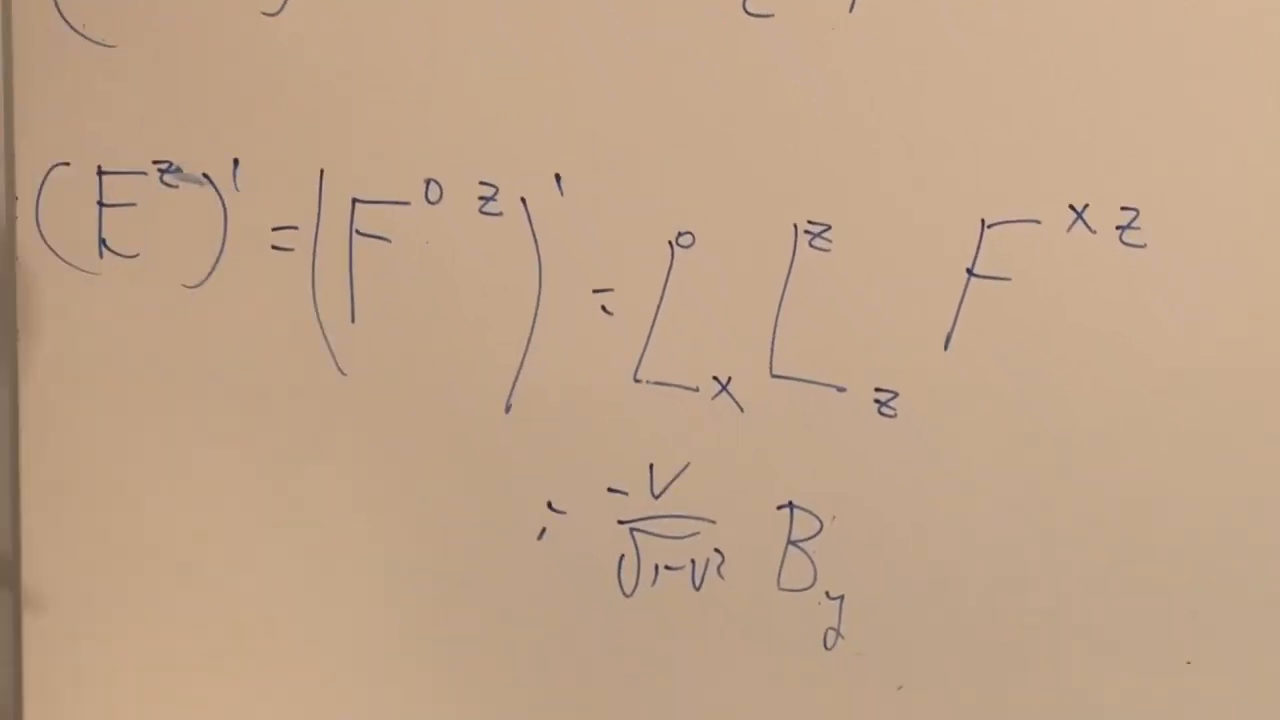
\includegraphics[width=\linewidth]{lecture_08_figure_07.png}
\caption{助推后选定的张量分量，显示因子\(\gamma v\)乘以原始磁分量。}
\par\smallskip
\textit{讲义帧：00:32:30。}
\end{figure}

选择加撇的参考系随电荷运动。电荷于是静止，因此其力的磁部分\(q\,\mathbf v'\times\mathbf B'\)不存在。然而力并未消失：它是\(q\mathbf E'\)。实验室观察者的磁力与共动观察者的电力是同一事件的两种描述。

这就是爱因斯坦第一段中谜题的答案。这个问题占据了本次讲座大约前四十分钟；历史笑话是它占据了爱因斯坦更长的时间。这个计算值得花时间，因为它将电场和磁场混合的口号转化为一个明确的张量分量。

\section{麦克斯韦方程组：恒等式与动力学}

现在从电荷上的力转向场方程。它们将在下一讲中从作用量推导出来。这里的目的首先是陈述它们，理解它们两种不同的逻辑角色，并将基于恒等式的那一半写成协变形式。

\begin{classroomqa}
\audiencequestion{我们不是已经推导出这些方程了吗？}
\lecturerresponse{我们推导的是带电粒子在给定电磁场中的运动方程。麦克斯韦方程则是场本身的运动方程，其中包含场对电荷和电流的响应。\lecturetimestamp{00:35:10}}
\end{classroomqa}

\begin{classroomqa}
\audiencequestion{麦克斯韦方程共有多少个？}
\lecturerresponse{共有八个标量分量方程。矢量记号将它们打包为两个标量方程和两个三分量矢量方程，习惯上称为四个麦克斯韦方程。\lecturetimestamp{00:35:24}}
\end{classroomqa}

我们继续使用这样的单位：\(c=1\)，并且通常的真空常数已被吸收到电荷和电流的定义之中。八个分量方程中有四个来自定义\(F=dA\)。它们是运动学恒等式。另外四个是动力学方程，如果场的作用量改变，它们就可能改变。

\subsection{三个基本矢量运算}

对于可微的三维矢量场\(\mathbf A\)，
\begin{align}
(\boldsymbol\nabla\times\mathbf A)_x
&=
\partial_yA_z-\partial_zA_y,
\\
\boldsymbol\nabla\cdot\mathbf A
&=
\partial_xA_x+\partial_yA_y+\partial_zA_z.
\end{align}
其余旋度分量可通过循环置换\(x\to y\to z\to x\)得到。对于标量场\(s\)，
\begin{equation}
\boldsymbol\nabla s
=
(\partial_xs,\partial_ys,\partial_zs).
\end{equation}
因此旋度是矢量，散度是标量，而梯度是矢量。

\begin{classroomqa}
\audiencequestion{有人需要完整复习旋度和散度的定义吗？}
\lecturerresponse{分量定义已经记录，但其余分量不必全部展开。循环置换坐标标号即可得到它们。\lecturetimestamp{00:37:32}}
\end{classroomqa}

光滑偏导数的可交换性给出两个恒等式：
\begin{align}
\boldsymbol\nabla\cdot
(\boldsymbol\nabla\times\mathbf A)
&=0,
\label{eq:div-curl}
\\
\boldsymbol\nabla\times
(\boldsymbol\nabla s)
&=\mathbf0.
\label{eq:curl-grad}
\end{align}

\begin{classroomqa}
\audiencequestion{我们是否应该写出旋度的散度为零的完整分量证明？}
\lecturerresponse{全班表示不必。展开分量会产生诸如\(\partial_x\partial_yA_z\)和
\(-\partial_y\partial_xA_z\)这样的项，它们因求导次序可以交换而相消。\lecturetimestamp{00:40:13}}
\end{classroomqa}

\begin{figure}[H]
\centering
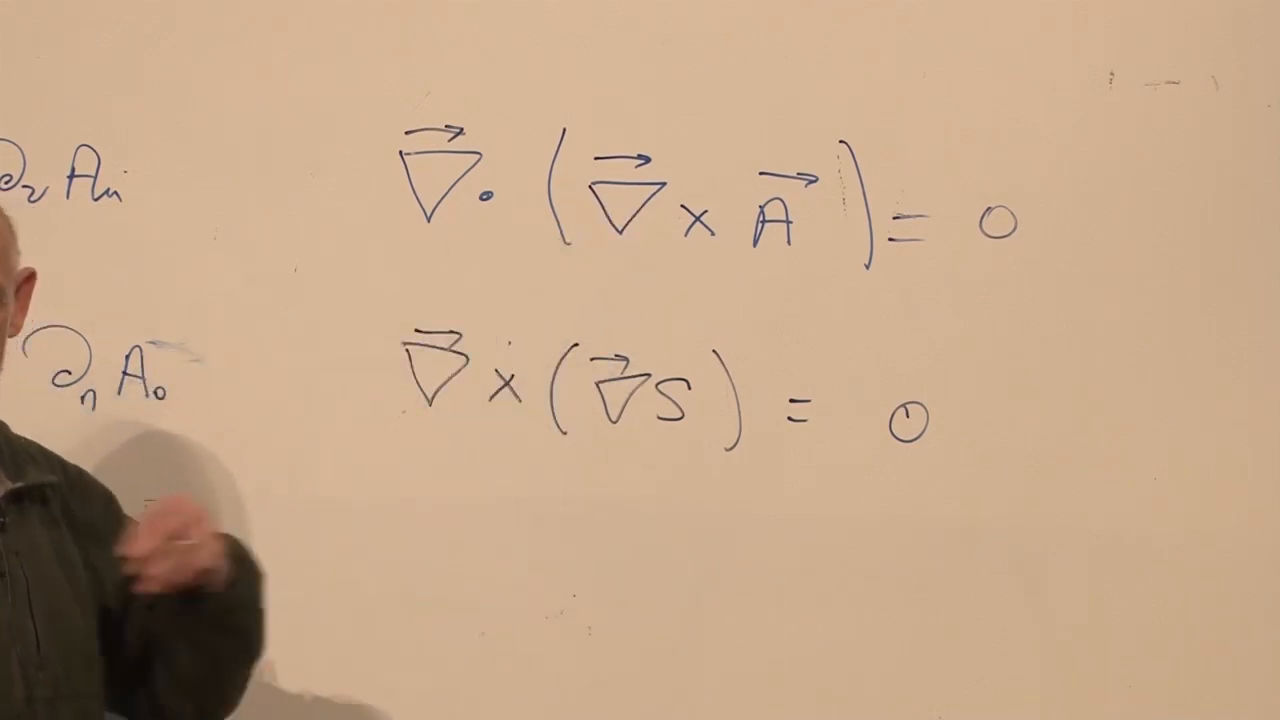
\includegraphics[width=\linewidth]{lecture_08_figure_08.png}
\caption{用于得到一半麦克斯韦方程的散度-旋度恒等式和梯度-旋度恒等式。}
\par\smallskip
\textit{讲义帧：00:41:40。}
\end{figure}

\subsection{矢量势不给出磁源}

对式~\eqref{eq:b-from-a}取散度，得到
\begin{equation}
\boldsymbol\nabla\cdot\mathbf B
=
\boldsymbol\nabla\cdot
(\boldsymbol\nabla\times\mathbf A)
=0.
\label{eq:div-b-zero}
\end{equation}
没有使用任何运动方程。该结果仅来自势的描述和光滑导数。

\begin{figure}[H]
\centering
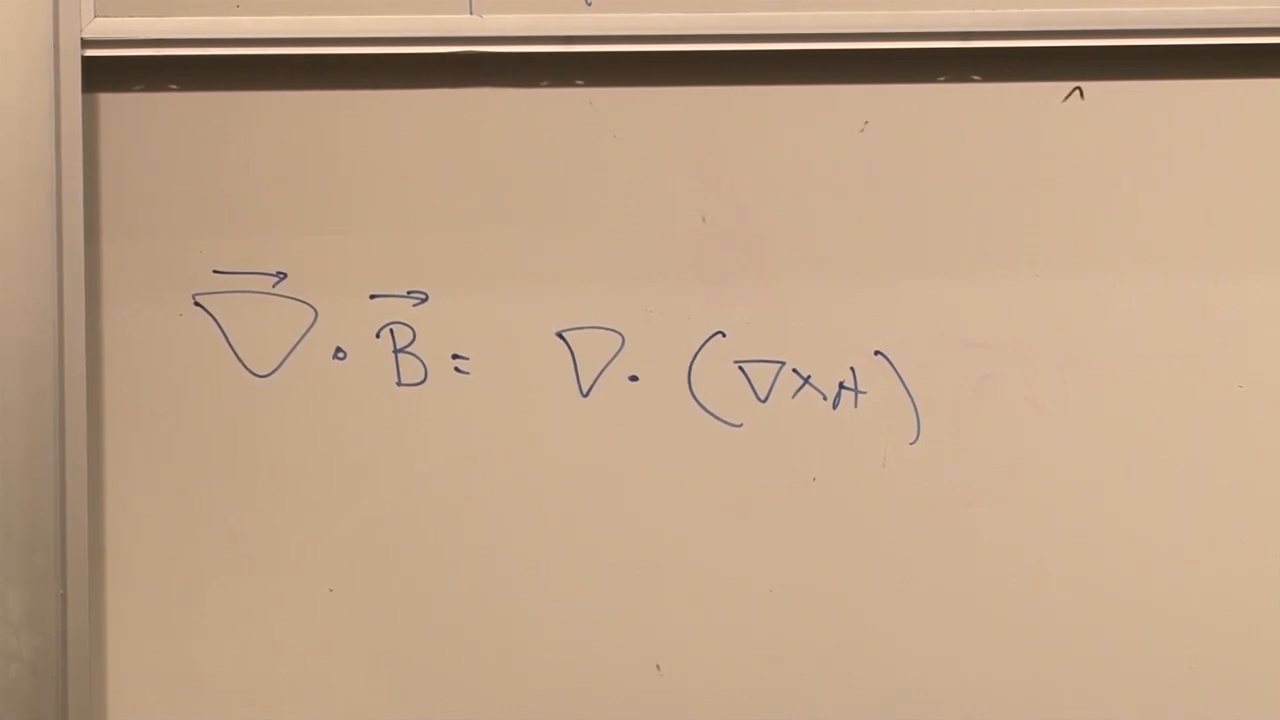
\includegraphics[width=\linewidth]{lecture_08_figure_09.png}
\caption{磁场的散度归结为一个旋度的散度。}
\par\smallskip
\textit{讲义帧：00:43:05。}
\end{figure}

\begin{classroomqa}
\audiencequestion{电场的散度是什么？}
\lecturerresponse{它是所用单位下的电荷密度，\(\boldsymbol\nabla\cdot\mathbf E=\rho\)。点电荷是电场线从源向外发散的典型情形。
\lecturetimestamp{00:43:20}}
\end{classroomqa}

在这个初等层面上，式~\eqref{eq:div-b-zero}说明不存在磁荷密度。一个光滑且整体定义的矢量势不能产生磁单极源。以后必须对这一陈述加以限定：磁单极可以用定义在重叠区域上的势或带有奇性的规范选择来描述。本讲推迟讨论这一改进。

\subsection{由电势得到法拉第方程}

式~\eqref{eq:e-from-a}用三维矢量记号写为
\begin{equation}
\mathbf E
=
\frac{\partial\mathbf A}{\partial t}
-\boldsymbol\nabla A_0.
\label{eq:e-vector-potential}
\end{equation}
尽管\(A_0\)属于一个四维矢量，但它在通常的空间旋转下是标量。取旋度：
\begin{align}
\boldsymbol\nabla\times\mathbf E
&=
\boldsymbol\nabla\times
\frac{\partial\mathbf A}{\partial t}
-
\boldsymbol\nabla\times
(\boldsymbol\nabla A_0)
\\
&=
\frac{\partial}{\partial t}
(\boldsymbol\nabla\times\mathbf A)
\\
&=
\frac{\partial\mathbf B}{\partial t}.
\end{align}
空间旋度与时间导数可交换，而梯度的旋度为零。

\begin{figure}[H]
\centering
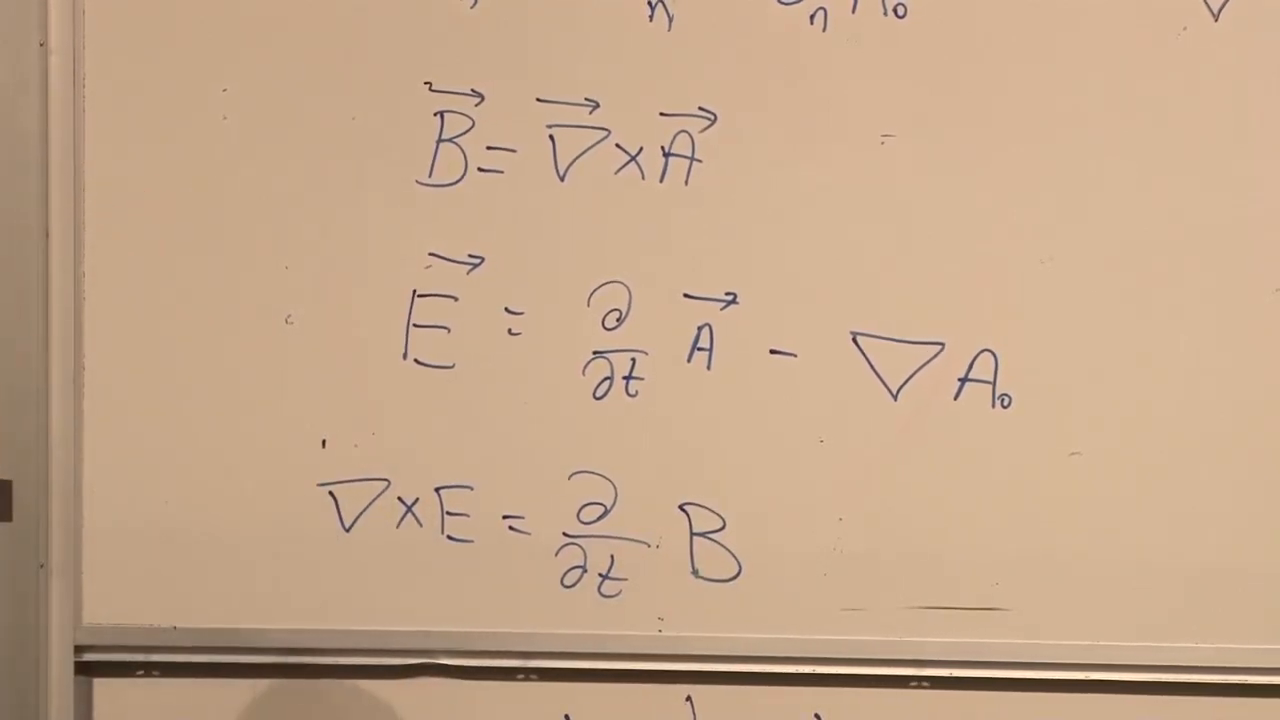
\includegraphics[width=\linewidth]{lecture_08_figure_10.png}
\caption{磁场的旋度、电势公式以及旋度计算的开端，构成一个完整的板书状态。}
\par\smallskip
\textit{讲义帧：00:47:45。}
\end{figure}

因此，四个齐次分量方程为
\begin{align}
\boldsymbol\nabla\cdot\mathbf B&=0,
\label{eq:homogeneous-div}
\\
\boldsymbol\nabla\times\mathbf E
-\frac{\partial\mathbf B}{\partial t}
&=\mathbf0.
\label{eq:homogeneous-curl}
\end{align}
第一个是一个标量方程；第二个是一个三分量矢量方程。

\begin{figure}[H]
\centering
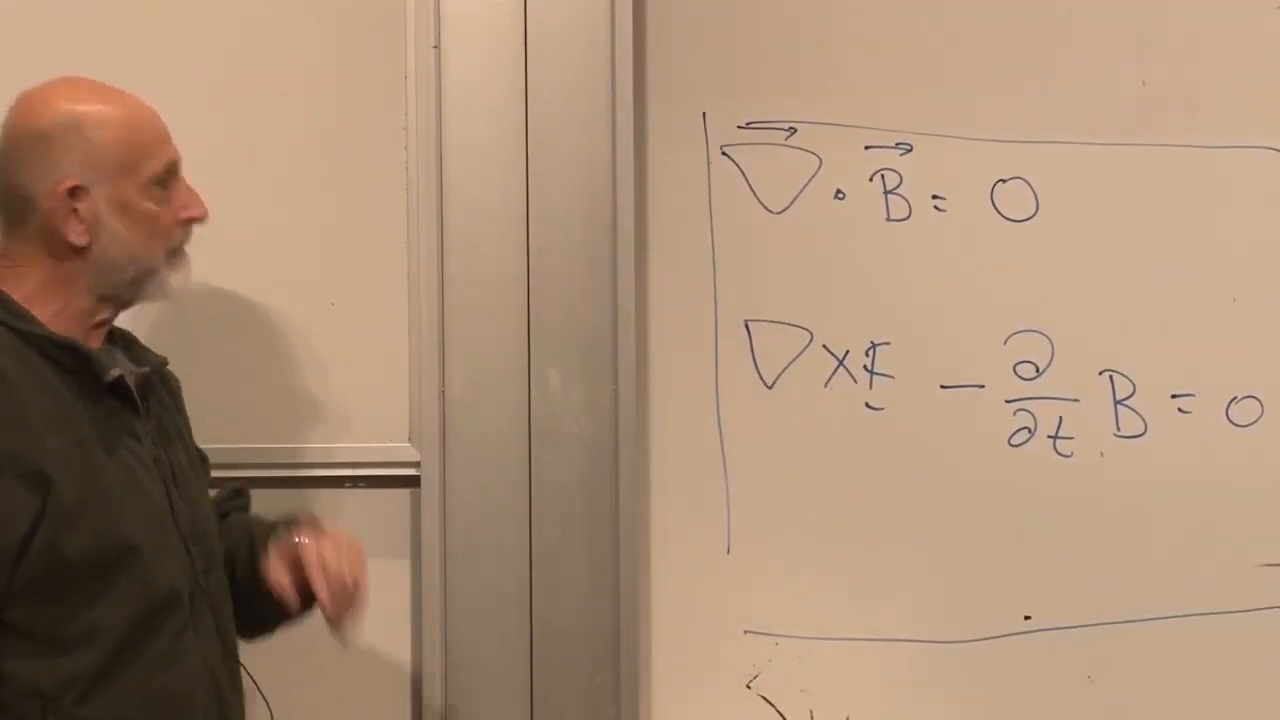
\includegraphics[width=\linewidth]{lecture_08_figure_11.png}
\caption{直接由势的定义得到的无源麦克斯韦方程组。}
\par\smallskip
\textit{讲义帧：00:48:45。}
\end{figure}

\subsection{动力学的一半}

其余方程为
\begin{align}
\boldsymbol\nabla\cdot\mathbf E&=\rho,
\label{eq:gauss-electric}
\\
\boldsymbol\nabla\times\mathbf B
+\frac{\partial\mathbf E}{\partial t}
&=-\mathbf J.
\label{eq:ampere-maxwell}
\end{align}
它们不是\(F=dA\)的推论。它们描述源如何产生和改变场，下一讲将从电磁作用量推导它们。电流项上的负号由已经选定的约定固定：\(F_{0i}=E_i\)、
\(F_{ij}=\epsilon_{ijk}B_k\)和
\(\partial_\mu F^{\mu\nu}=J^\nu\)。现场板书最初把\(\mathbf J\)放在右边而没有这个负号；由此产生的与电荷守恒的不一致将在下一讲中被注意到并纠正。

\begin{classroomqa}
\audiencequestion{旋度方程右侧是什么类型的量？}
\lecturerresponse{左侧是一个三维矢量，因此右侧也是一个三维矢量，称为电流密度\(\mathbf J\)。高斯方程右侧是三维标量电荷密度\(\rho\)。
\lecturetimestamp{00:50:36}}
\end{classroomqa}

\begin{figure}[H]
\centering
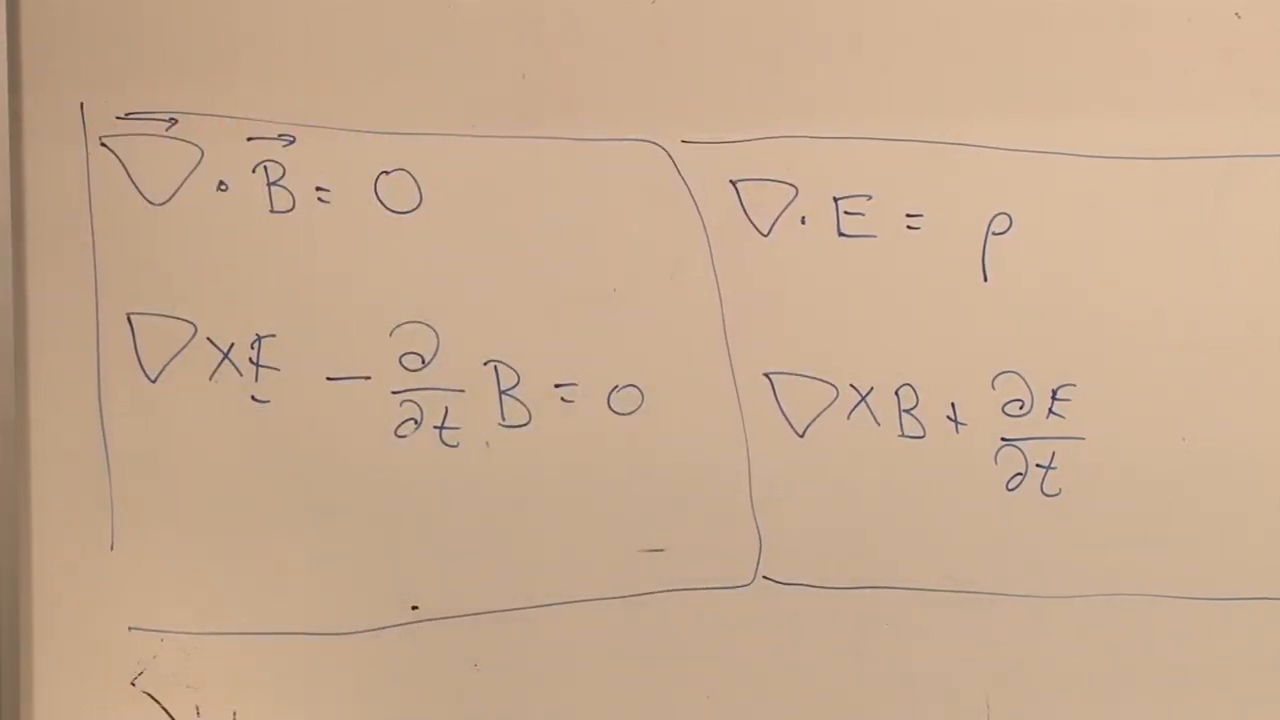
\includegraphics[width=\linewidth]{lecture_08_figure_12.png}
\caption{四个麦克斯韦方程分为基于恒等式的一对和有源动力学的一对。}
\par\smallskip
\textit{讲义帧：00:50:40。}
\end{figure}

\section{电荷与电流作为时空流}

符号\(\rho\)和\(\mathbf J\)现在必须被赋予几何意义。电荷密度是单位体积内的电荷；电流密度是单位时间内穿过有向面积的电荷。讲义从世界线出发推导两者，以便它们后来统一为四维矢量时不会显得偶然。

\subsection{来自邻室黑板的一段课堂插话}

在绘制那些世界线之前，邻室中可见的方程引出了一段简短的教学插话。一门即将开设的课程将向数学系教师介绍量子力学，他们希望获得量子场论及其与现代数学联系所需的背景知识。挑战是双向的：物理学家必须把隐含的物理习惯明确表达出来，而数学家必须了解那些形式结构被要求描述的是什么。

\begin{classroomqa}
\audiencequestion{谁会被认为觉得这项教学任务令人沮丧？}
\lecturerresponse{可能双方都是：物理学家要教一群不熟悉的听众，而数学家要面对形式体系背后的物理习惯。不过这项任务预计会很有趣。随后课堂回到电荷与电流。\lecturetimestamp{00:53:20}}
\end{classroomqa}

\subsection{电荷密度}

把时间画成竖直方向，让其余画出的方向代表三维空间。带电粒子描出世界线。在某一固定时刻，放置一个体积为\(\Delta V\)的小空间立方体横跨那束世界线，并把它内部粒子的电荷相加。电荷密度为
\begin{equation}
\rho(t,\mathbf x)
=
\lim_{\Delta V\to0}
\frac{\Delta Q}{\Delta V}.
\label{eq:charge-density}
\end{equation}
黑板上的二维正方形代表一个三维立方体；缺少的那个空间方向之所以被省略，只是因为四维无法画在平面黑板上。

\begin{figure}[H]
\centering
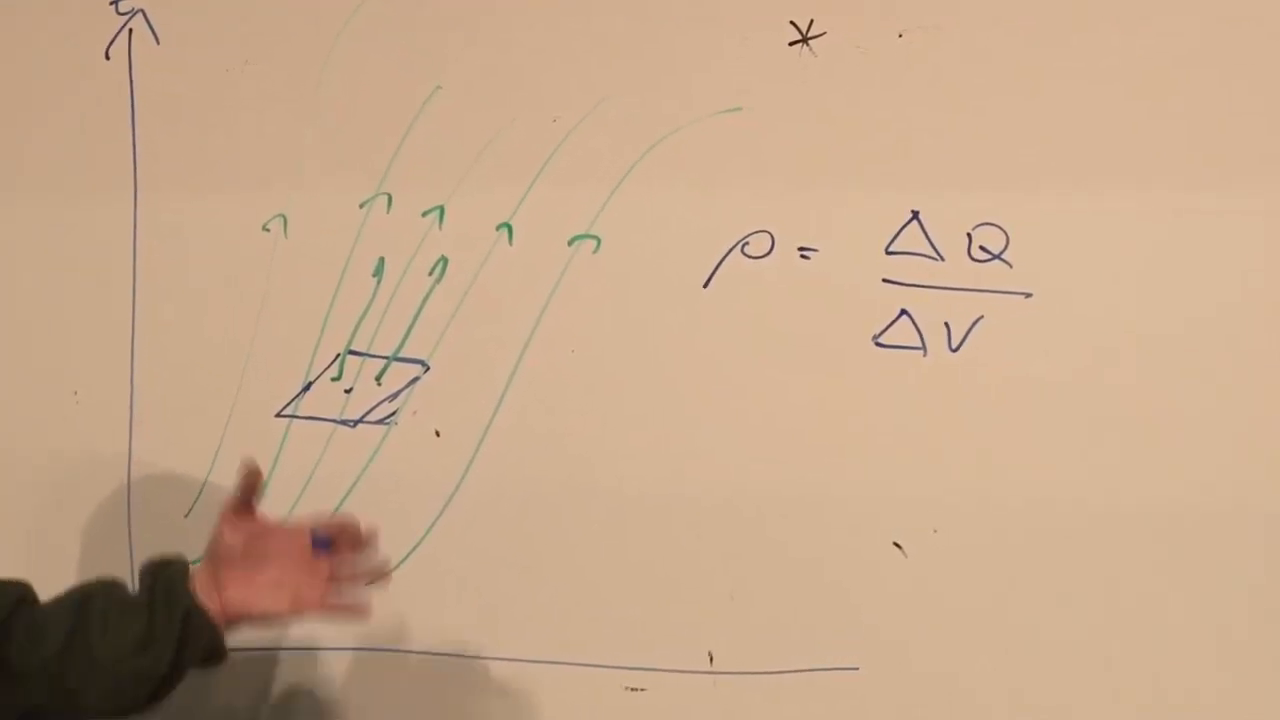
\includegraphics[width=\linewidth]{lecture_08_figure_13.png}
\caption{带电粒子世界线穿过一个小空间元胞，其中\(\rho=\Delta Q/\Delta V\)。}
\par\smallskip
\textit{讲义帧：00:57:20。}
\end{figure}

\subsection{电流密度}

把时空元胞侧过来。为了定义\(J_x\)，在\(yz\)平面内选择一个面积为\(\Delta A_x\)的小窗口，垂直于\(x\)轴。数出在\(\Delta t\)期间从负\(x\)侧穿过到正\(x\)侧的净电荷：
\begin{equation}
J_x
=
\lim_{\Delta A_x,\Delta t\to0}
\frac{\Delta Q_x}{\Delta A_x\,\Delta t}.
\label{eq:jx-window}
\end{equation}
取向给出符号。垂直于\(y\)和\(z\)的窗口以同样方式定义\(J_y\)和\(J_z\)。

黑板诚实地面对作图的困难：\(yz\)平面内的窗口看起来像天花板上的窗口，而不是墙上的窗口。相关的轴就是比一次能显示出来的更多。即使草图并非如此，不变的定义也是明确的。

\begin{classroomqa}
\audiencequestion{图中的窗口是在天花板上吗？}
\lecturerresponse{在房间类比中，是的。重要的是它的平面垂直于\(x\)方向。一个\(yz\)面积度量穿过它的\(x\)方向电流。\lecturetimestamp{00:59:38}}
\end{classroomqa}

\begin{figure}[H]
\centering
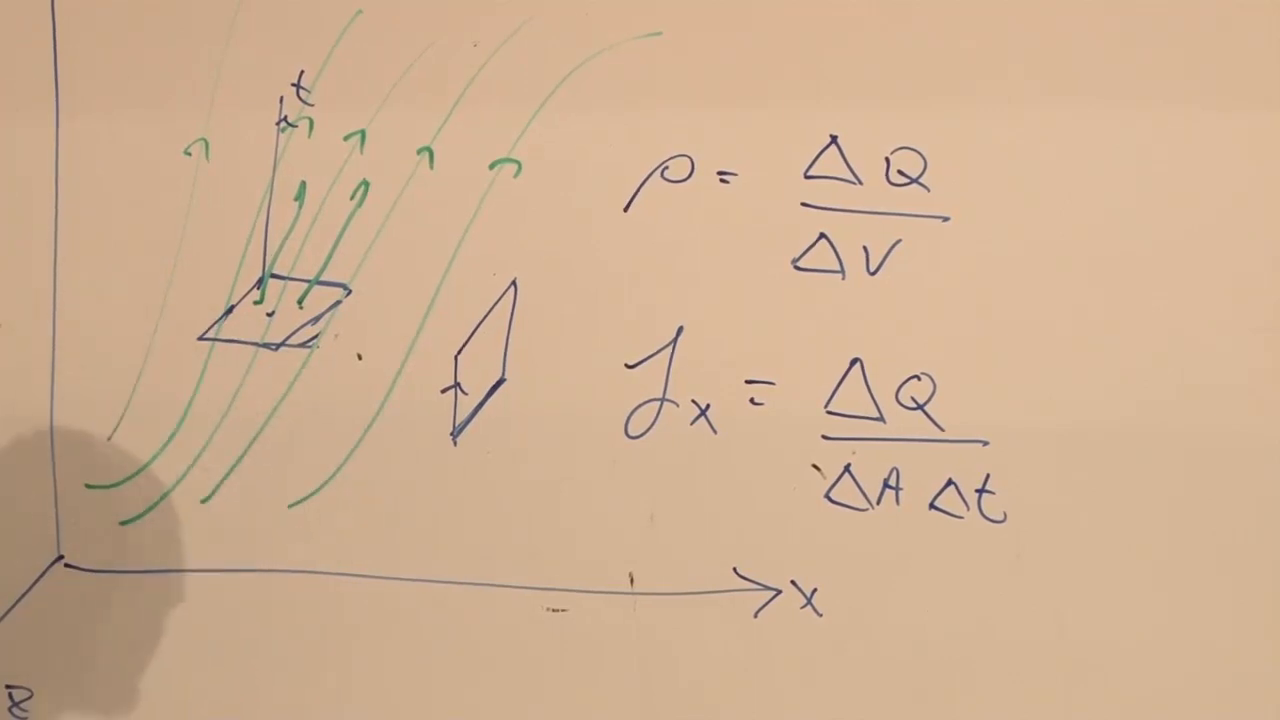
\includegraphics[width=\linewidth]{lecture_08_figure_14.png}
\caption{电荷电流穿过横向窗口，其中\(J_x=\Delta Q/(\Delta A\,\Delta t)\)。}
\par\smallskip
\textit{讲义帧：01:01:40。}
\end{figure}

\begin{figure}[H]
\centering
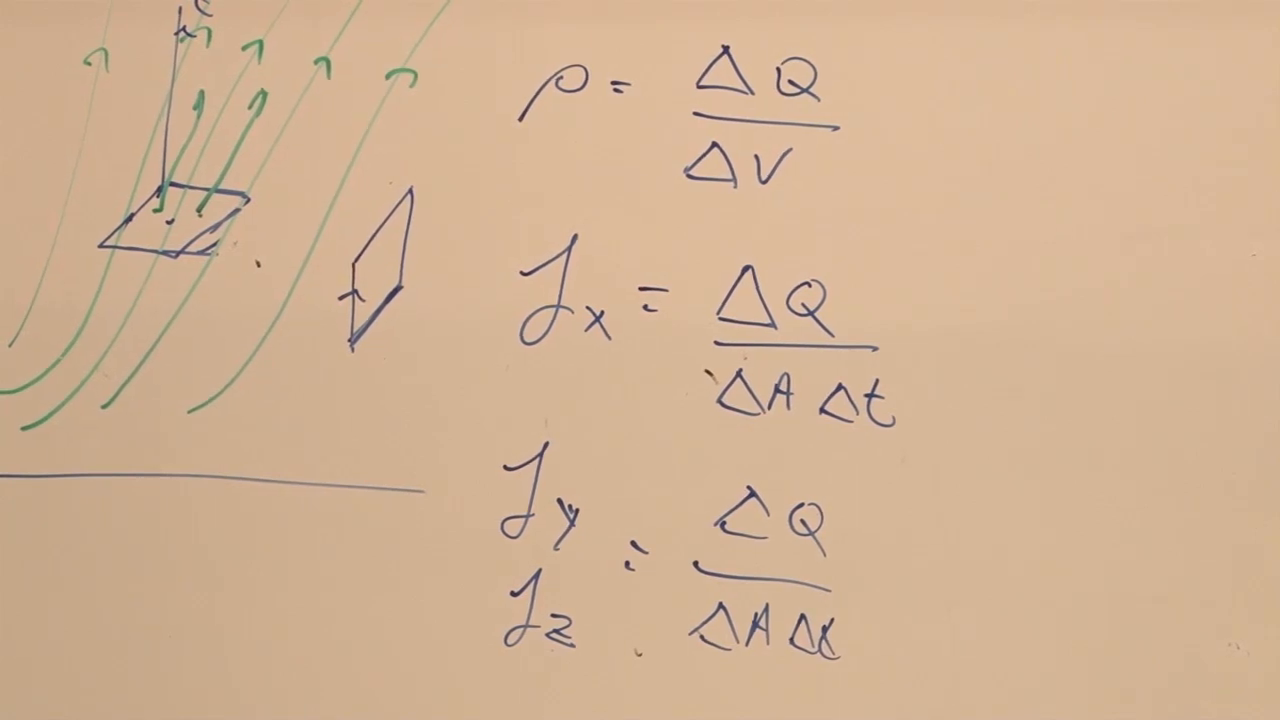
\includegraphics[width=\linewidth]{lecture_08_figure_15.png}
\caption{由电荷穿过垂直于三个空间轴的窗口所定义的三个电流分量。}
\par\smallskip
\textit{讲义帧：01:02:40。}
\end{figure}

这四个量有平行的定义。某一瞬间的空间体积是垂直于时间轴的超曲面，因此\(\rho\)是电荷穿过时间法向窗口的流。\(J_i\)是穿过空间法向窗口的流。

\begin{classroomqa}
\audiencequestion{这四个数是一个沿时间方向的流和三个沿空间方向的流吗？}
\lecturerresponse{这正是有用的图像。空间体积是垂直于时间轴的窗口；三个横向面积是垂直于\(x\)、\(y\)和\(z\)的窗口。它们的四个通量属于一起。\lecturetimestamp{01:04:14}}
\end{classroomqa}

这提示了逆变四维电流
\begin{equation}
J^\mu
=
(\rho,J_x,J_y,J_z).
\label{eq:four-current}
\end{equation}

\begin{classroomqa}
\audiencequestion{度规从哪里进入，而这个流是协变的还是逆变？}
\lecturerresponse{按这里的定义，\(\rho\) 与三个 \(J_i\) 构成 \(J^\mu\) 的分量，即一个上指标或逆变四维矢量。当需要 \(J_\mu\) 时，度规将其指标降低。协变形式的麦克斯韦表述将说明为什么选择上指标是自然的。
\lecturetimestamp{01:04:48}}
\end{classroomqa}

\section{休息时的插曲：黑洞附近的信号}

到了预定的休息时间，问题转向先前关于黑洞的讨论。虽然这是对电动力学的离题，但它是课堂上一次实质性的交流，并且说明了同一种训练：区分不同观测者所作的描述。

\begin{classroomqa}
\audiencequestion{如果远处观测者看到下落物体在视界附近变慢，那么黑洞是否应该看起来被曾经落到它上面的一切所覆盖？}
\lecturerresponse{在施瓦西坐标时中，经典下落被看作渐近地趋近视界。人们可以把相继的物质想象成在视界附近越来越被压缩的层。然而在操作上，出射信号越来越延迟、红移并且微弱。以普通局部频率发出的光首先以可见光到达，然后是红外、微波和射电，每个光子携带的能量都更少。没有任何现实的远处探测器会永远看到一个明亮的冻结物体；它逐渐消失在黑暗中。
\lecturetimestamp{01:06:11}}
\end{classroomqa}

下落观测者的钟和局部发出的手电筒光对该观测者来说仍是普通的。远处的描述不同，因为频率和到达率都发生了红移。在有限能量和有限带宽下，信息实际上存在最后一个可分辨的部分。

\begin{classroomqa}
\audiencequestion{物体是在渐近地趋近事件视界吗？}
\lecturerresponse{这就是远处的施瓦西坐标描述。在量子力学上，还必须把逐渐消逝的信号与黑洞的霍金辐射区分开来。在足够晚的时刻，微弱的红移信号在黑洞自身辐射的背景中从观测上丢失了。\lecturetimestamp{01:09:24}}
\end{classroomqa}

\begin{classroomqa}
\audiencequestion{如果红移后的波长增长到超过可观测宇宙的尺度，会怎样？}
\lecturerresponse{远在那之前，信号实际上就已经丢失了。讲座给出了霍金的量级图像：大约每个光穿越时间一个典型量子，
\[
t_{\rm cross}\sim\frac{R_s}{c}.
\]
对于一个大黑洞，这是极其微弱的辐射，而一个红移足够大的下落信号会远早于任何宇宙学波长界限而变得不可探测。\lecturetimestamp{01:09:50}}
\end{classroomqa}

\begin{classroomqa}
\audiencequestion{大约每个穿越时间一个量子的速率在黑洞的整个寿命中保持不变吗？}
\lecturerresponse{不。一个蒸发的施瓦西黑洞会收缩，所以它的穿越时间减少，霍金温度升高。因此发射会加速。用瞬时半径表示的维度估计仍然有用，但半径不是常数。相应地，典型的霍金波长随着蒸发进行而变短。\lecturetimestamp{01:11:42}}
\end{classroomqa}

休息之后，脱去夹克，我们回到 \(\rho\) 和 \(\mathbf J\)。

\section{电荷的局域守恒}

人们很容易只把电荷守恒表述为
\begin{equation}
\frac{dQ_{\rm universe}}{dt}=0.
\end{equation}
这种表述太弱了。电荷可能从一个实验室消失并瞬间在半人马座{\proseunicodefont α}星重新出现，或者在更远的后发星系团中重新出现，而总量不变。这样的定律几乎没有实验约束力。

更强的表述是局域的：一个区域内的电荷只能通过穿过该区域的边界而改变。在一点周围放置一个小盒子。如果它的电荷增加，那么通过其六个面必定有净向内的电流；如果减少，则必定有净向外的电流。

\subsection{通过相对面的通量}

取垂直于 \(x\) 的两个面。一个面上的向内贡献在 \(x\) 的一个值处计算；相对面上的贡献在相距一小段距离处计算。它们的差除以盒子宽度，趋近于
\begin{equation}
-\partial_xJ_x.
\end{equation}
出现负号是因为正的 \(J_x\) 被定义为朝向 \(x\) 增大的方向流动，而向外的通量会减少盒子中的电荷。\(y\) 面和 \(z\) 面这两对类似地贡献
\(-\partial_yJ_y\) 和 \(-\partial_zJ_z\)。因此
\begin{equation}
\frac{\partial\rho}{\partial t}
=
-\partial_xJ_x-\partial_yJ_y-\partial_zJ_z
=
-\boldsymbol\nabla\cdot\mathbf J.
\end{equation}
等价地，
\begin{equation}
\boxed{
\frac{\partial\rho}{\partial t}
+\boldsymbol\nabla\cdot\mathbf J=0
}.
\label{eq:continuity}
\end{equation}

\begin{figure}[H]
\centering
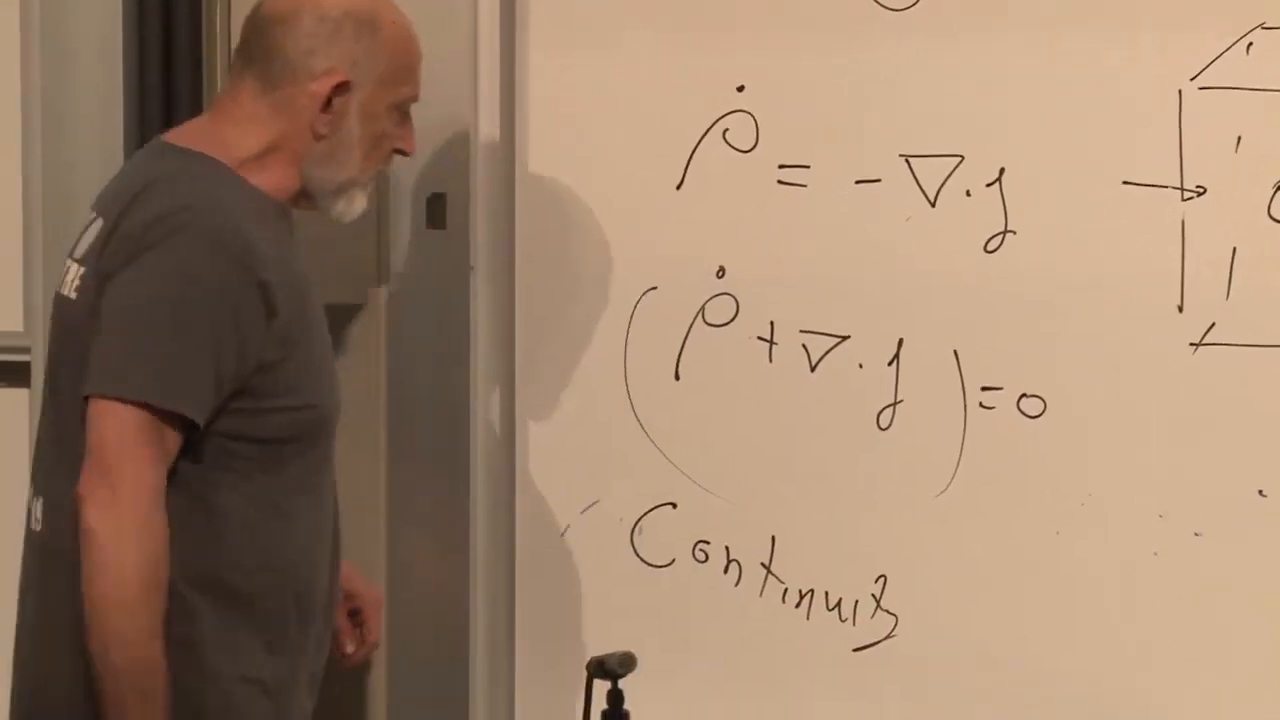
\includegraphics[width=\linewidth]{lecture_08_figure_16.png}
\caption{局部平衡定律
\(\dot\rho=-\boldsymbol\nabla\cdot\mathbf J\)，以及边界电流产生该定律的小盒子。}
\par\smallskip
\textit{讲义帧：01：20：45。}
\end{figure}

这通常被称为连续性方程。讲义更倾向于称之为\emph{局部守恒}：连续性可能暗示一种数学上的光滑性假设，而物理内容则是电荷不能在这里消失、又在那里出现，除非两者之间有电流。

\subsection{为什么麦克斯韦需要位移电流}

方程~\eqref{eq:continuity}并非麦克斯韦方程组的独立补充。对高斯定律取时间导数，对安培--麦克斯韦定律取散度：
\begin{align}
\frac{\partial\rho}{\partial t}
&=
\boldsymbol\nabla\cdot
\frac{\partial\mathbf E}{\partial t},
\\
-\boldsymbol\nabla\cdot\mathbf J
&=
\boldsymbol\nabla\cdot
(\boldsymbol\nabla\times\mathbf B)
+
\boldsymbol\nabla\cdot
\frac{\partial\mathbf E}{\partial t}
\\
&=
\boldsymbol\nabla\cdot
\frac{\partial\mathbf E}{\partial t}.
\end{align}
因此两个左边相等，给出
\(\partial_t\rho=-\boldsymbol\nabla\cdot\mathbf J\)，正是方程~\eqref{eq:continuity}。结构上重要的是，\(\mathbf E\)的时间导数，即位移电流项，对于散度关系与电荷守恒相容是必不可少的。

\begin{classroomqa}
\audiencequestion{我们还没有说明两个有源麦克斯韦方程从何而来，对吧？}
\lecturerresponse{没有。它们是动力学目标，下次将从作用量推导出来。静磁旋度定律在麦克斯韦之前就已为人所知；麦克斯韦关键的时间相关补充是位移电流。它的存在使场方程与局部电荷守恒相容。\lecturetimestamp{01:23:15}}
\end{classroomqa}

详细的散度计算在讲义中留作练习，但其结论并非可有可无：麦克斯韦方程组要求电荷守恒。

\section{四维电流及其散度}

将方程~\eqref{eq:continuity}写成各分量：
\begin{equation}
\frac{\partial\rho}{\partial t}
+
\frac{\partial J_x}{\partial x}
+
\frac{\partial J_y}{\partial y}
+
\frac{\partial J_z}{\partial z}
=0.
\label{eq:continuity-components}
\end{equation}

\begin{figure}[H]
\centering
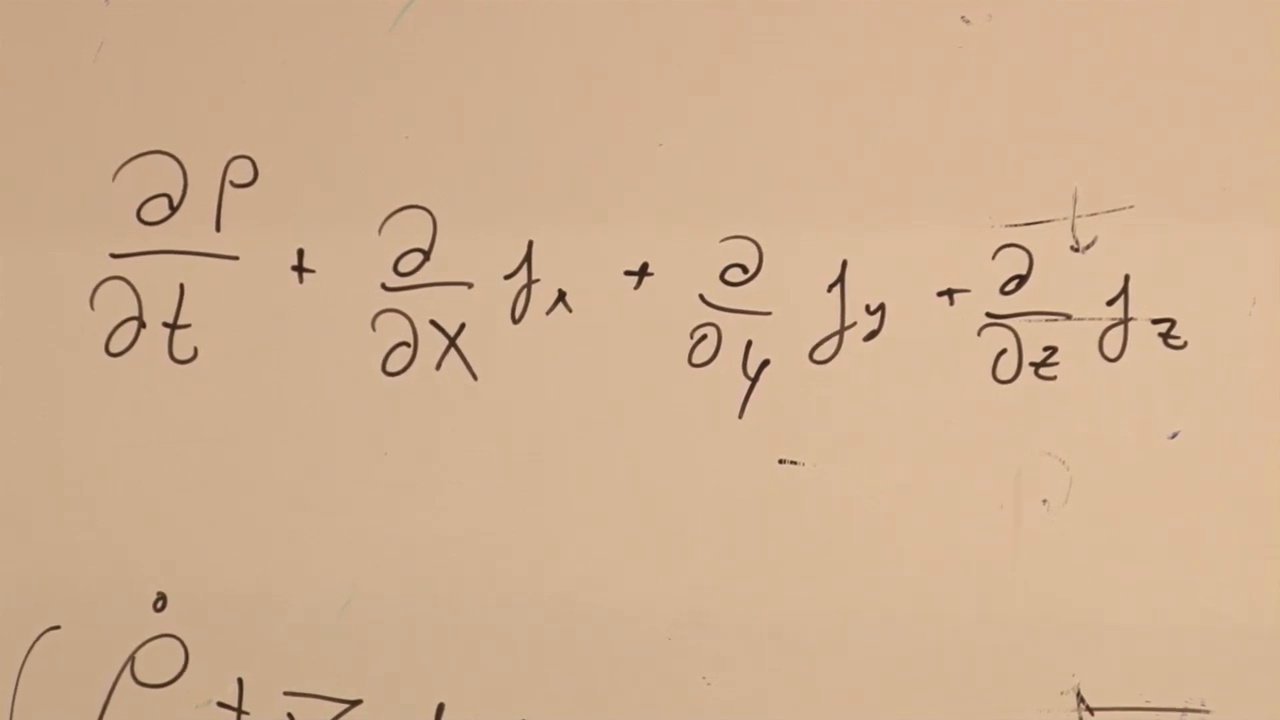
\includegraphics[width=\linewidth]{lecture_08_figure_17.png}
\caption{局部电荷守恒展开为一个时间导数和三个空间导数。}
\par\smallskip
\textit{讲义帧：01：25：40。}
\end{figure}

由方程~\eqref{eq:four-current}定义\(J^\mu\)后，这四项就是一次缩并：
\begin{equation}
\boxed{\partial_\mu J^\mu=0}.
\label{eq:four-current-conservation}
\end{equation}
\(\partial_\mu\)上的下指标与\(J^\mu\)上的上指标缩并，因此结果是洛伦兹标量。几何窗口的构造已经暗示了这一变换律：\(\rho\)与三个电流分量是同一电荷通量的四种取向。

\begin{figure}[H]
\centering
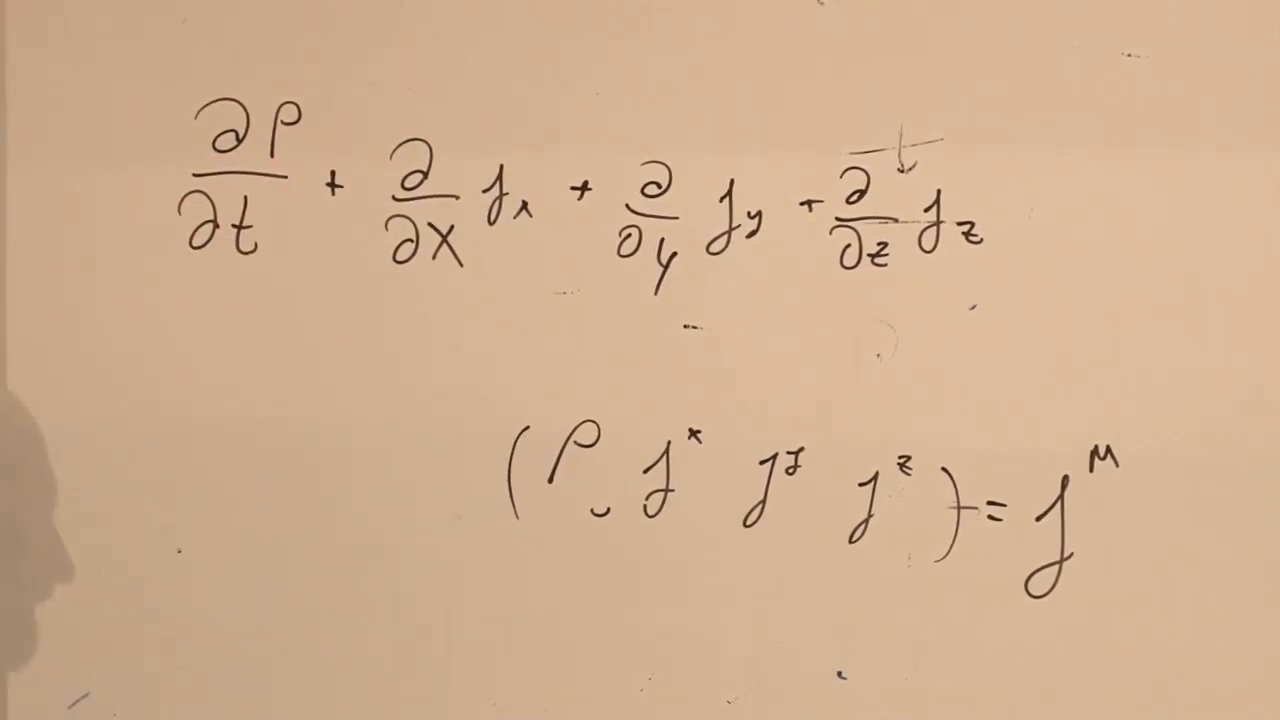
\includegraphics[width=\linewidth]{lecture_08_figure_18.png}
\caption{分量\((\rho,J_x,J_y,J_z)\)组装成\(J^\mu\)并与四维梯度缩并。}
\par\smallskip
\textit{讲义帧：01：27：10。}
\end{figure}

\begin{classroomqa}
\audiencequestion{\(\rho\)的时间导数何时变成了偏导数？}
\lecturerresponse{它从一开始就是偏导数。我们保持空间盒子固定，并询问其电荷密度随时间变化如何改变。我们并不是在跟随一条运动轨迹，所以这里的\(\dot\rho\)指的是在固定\(x,y,z\)下的\(\partial\rho/\partial t\)。
\lecturetimestamp{01:28:20}}
\end{classroomqa}

\section{协变形式的齐次方程}

我们现在拥有了所需的客体：
\begin{itemize}
\item \(\mathbf E\)和\(\mathbf B\)是反对称张量\(F_{\mu\nu}\)的六个独立分量；
\item \(\rho\)和\(\mathbf J\)是\(J^\mu\)的四个分量；
\item 局部守恒是标量方程
\(\partial_\mu J^\mu=0\)。
\end{itemize}
本讲剩余的任务是把齐次麦克斯韦方程组，即方程~\eqref{eq:homogeneous-div}和
\eqref{eq:homogeneous-curl}，写成一个张量方程。

\subsection{循环导数}

答案是
\begin{equation}
\boxed{
\partial_\sigma F_{\nu\tau}
+
\partial_\nu F_{\tau\sigma}
+
\partial_\tau F_{\sigma\nu}
=0
}.
\label{eq:bianchi}
\end{equation}
这三项循环地分配导数指标和两个场张量指标。这常缩写为
\begin{equation}
\partial_{[\sigma}F_{\nu\tau]}=0,
\end{equation}
其中方括号表示反对称化。

\begin{figure}[H]
\centering
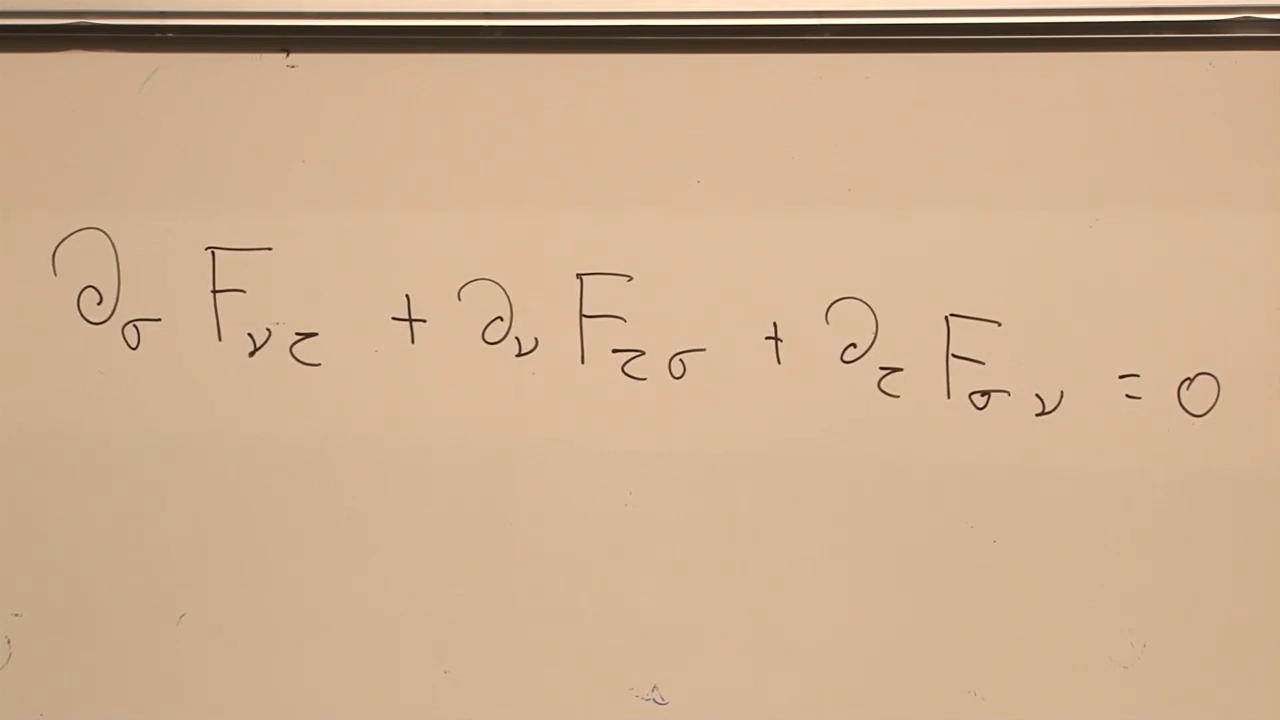
\includegraphics[width=\linewidth]{lecture_08_figure_19.png}
\caption{将齐次麦克斯韦方程打包在一起的循环三指标方程。}
\par\smallskip
\textit{讲义帧：01：33：20。}
\end{figure}

\subsection{三个指标全为空间指标}

令
\begin{equation}
(\sigma,\nu,\tau)=(x,y,z).
\end{equation}
则
\begin{align}
0
&=
\partial_xF_{yz}
+
\partial_yF_{zx}
+
\partial_zF_{xy}
\\
&=
\partial_xB_x+\partial_yB_y+\partial_zB_z
\\
&=
\boldsymbol\nabla\cdot\mathbf B.
\end{align}
因此方程~\eqref{eq:bianchi}的全空间分量正是磁散度为零。

\begin{figure}[H]
\centering
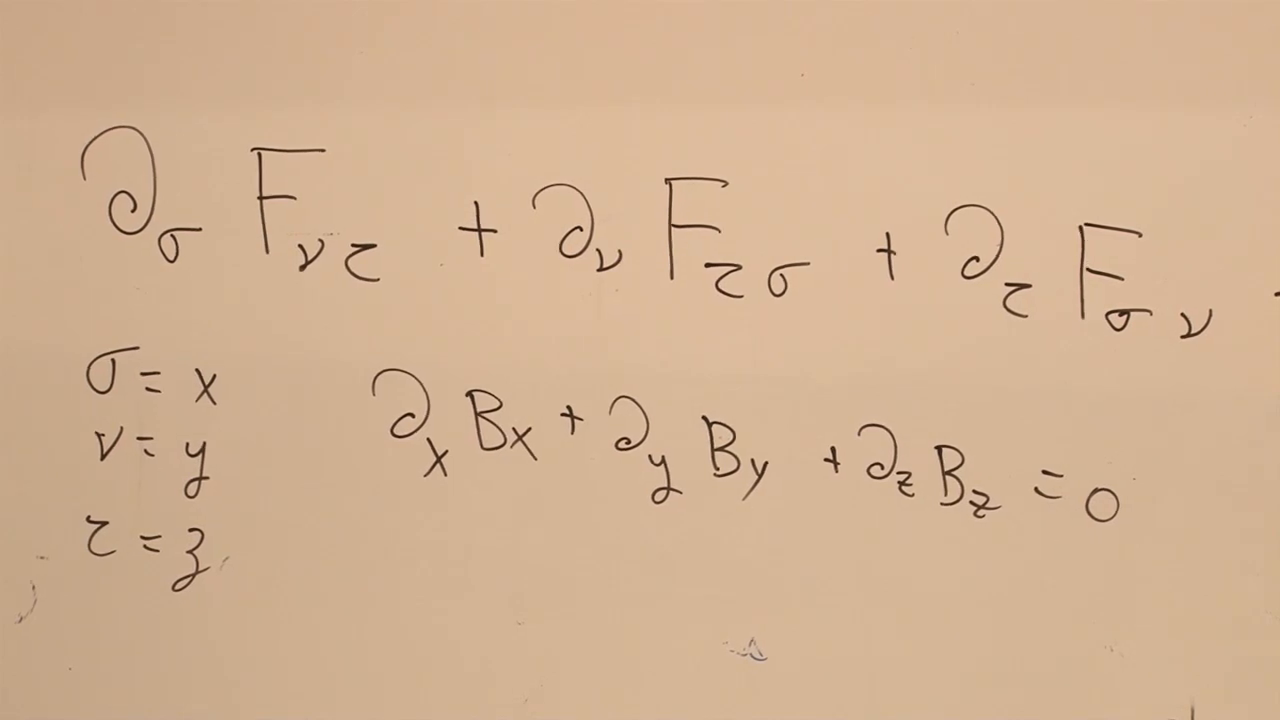
\includegraphics[width=\linewidth]{lecture_08_figure_20.png}
\caption{循环恒等式的全空间分量约化为\(\partial_xB_x+\partial_yB_y+\partial_zB_z=0\)。}
\par\smallskip
\textit{讲义帧：01：35：30。}
\end{figure}

\subsection{一个时间指标}

例如选择
\begin{equation}
(\sigma,\nu,\tau)=(y,x,0).
\end{equation}
则方程~\eqref{eq:bianchi}将电场分量的两个空间导数与磁场分量的一个时间导数组合起来：
\begin{equation}
\partial_yF_{x0}
+
\partial_xF_{0y}
+
\partial_0F_{yx}
=0.
\end{equation}
利用方程~\eqref{eq:f-lower-matrix}中的矩阵，这是
\begin{equation}
\boldsymbol\nabla\times\mathbf E
-\frac{\partial\mathbf B}{\partial t}
=\mathbf0,
\end{equation}
的一个分量，其相对符号由反对称性固定。选择其他空间指标对则给出另外两个旋度分量。

\begin{figure}[H]
\centering
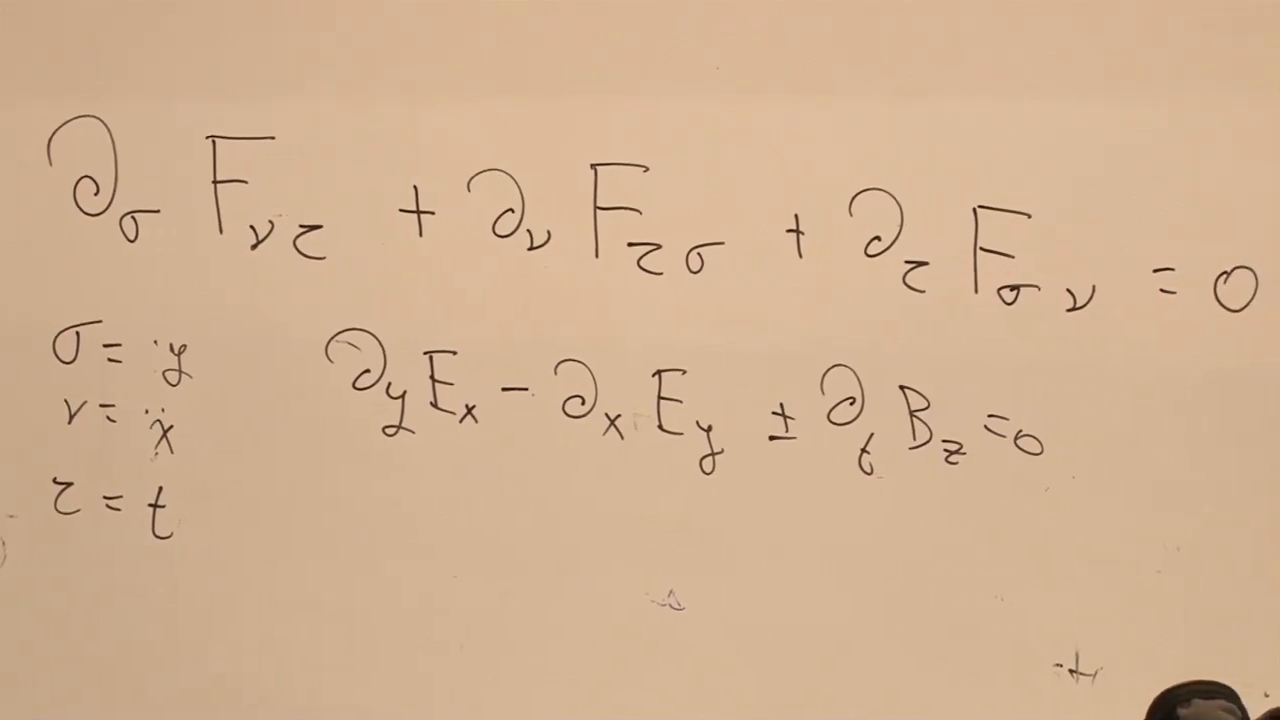
\includegraphics[width=\linewidth]{lecture_08_figure_21.png}
\caption{一次性的、双空格的张量分量检查，给出法拉第方程的一个分量。}
\par\smallskip
\textit{讲义帧：01:38:20。}
\end{figure}

还有一个直接证明。将方程~\eqref{eq:field-tensor-definition}代入方程~\eqref{eq:bianchi}。会出现六个二阶导数项，它们两两相消，因为偏导数可交换。这是散度之旋度和梯度之旋度恒等式的四维版本。

\begin{classroomqa}
\audiencequestion{Bianchi 这个名字里有一个 \(h\) 吗？}
\lecturerresponse{有。这个循环方程就是电磁 Bianchi 恒等式，它是一个几何恒等式的特例，该恒等式也出现在广义相对论中。其更深刻的几何解释留待以后讨论。
\lecturetimestamp{01:40:28}}
\end{classroomqa}

\subsection{为什么写出的六十四个分量只包含四个方程}

三个指标，每个都有四个可能取值，看起来会产生
\(4^3=64\) 个方程。反对称性消除了冗余：
\begin{itemize}
\item 如果任意两个指标相同，循环表达式恒为零；
\item 如果三个指标全都不同，置换会重现同一个方程，至多相差一个符号；
\item 四维中只有
\(\binom{4}{3}=4\) 个由互不相同指标构成的无序三元组。
\end{itemize}
共有 \(24\) 个所有指标互不相同的有序三元组，它们分成四组、每组六个置换。其余 \(40\) 个有序三元组为零。这四个独立方程是一个磁散度方程和法拉第方程的三个分量。

\begin{classroomqa}
\audiencequestion{场张量有六个独立分量，但三指标表达式似乎包含六十四个方程。为什么只剩下四个？}
\lecturerresponse{重复指标给出零，而三个不同指标的置换会重复同一个关系，至多相差一个符号。因此，表面上六十四个分量坍缩为四个独立方程。
\lecturetimestamp{01:41:58}}
\end{classroomqa}

方程~\eqref{eq:bianchi}显然是张量性的，因此是洛伦兹协变的。在光滑的单势描述中，它还表明既没有磁荷密度，也没有磁流。有源的动力学配对恰好停留在本讲所达到的边界：其协变方程和作用的推导属于下一次课。

\section{对偶性与磁单极子问题}

最后的问题回到电源与磁源之间表面上的不对称性。在真空中，麦克斯韦方程组具有电--磁对偶旋转
\begin{equation}
\mathbf E\longrightarrow\mathbf B,
\qquad
\mathbf B\longrightarrow-\mathbf E.
\label{eq:duality-quarter-turn}
\end{equation}
这是在以 \(\mathbf E\) 和 \(\mathbf B\) 为轴的抽象平面中的一个九十度旋转，而不是仅仅交换二者标签的反射。当电源和磁源同时存在时，电四维流和磁四维流必须同时旋转。

\begin{figure}[H]
\centering
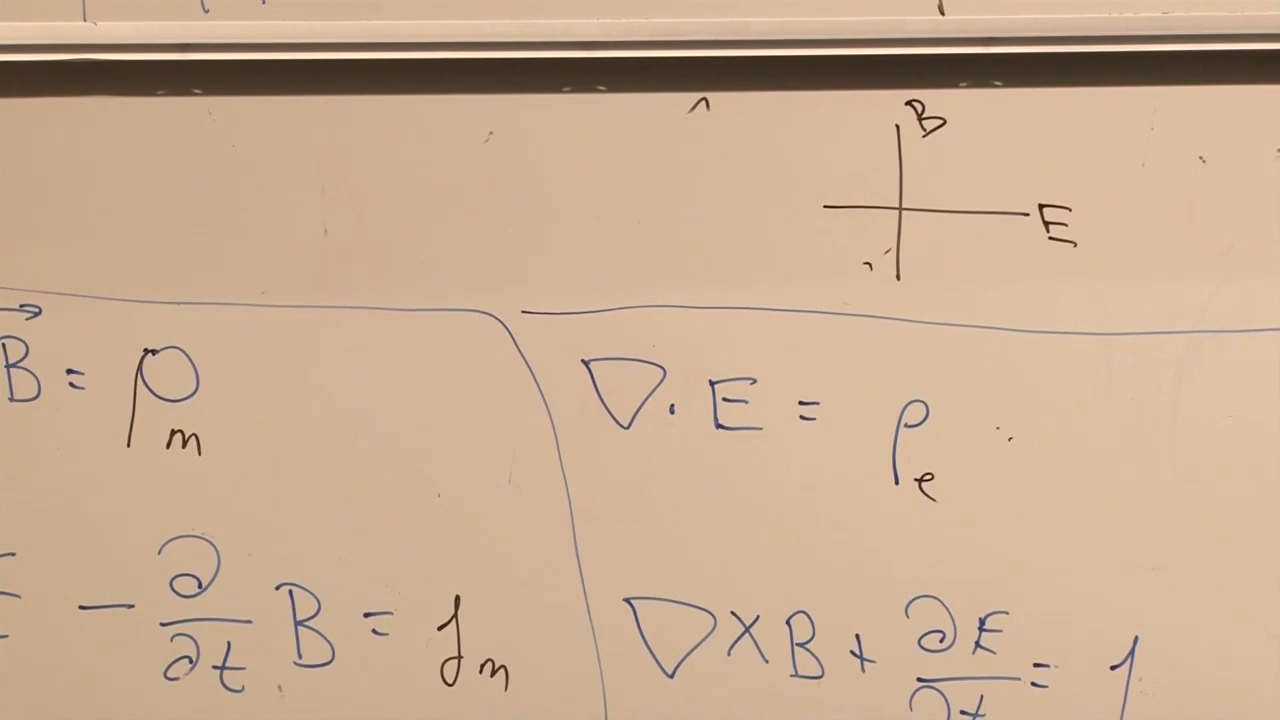
\includegraphics[width=\linewidth]{lecture_08_figure_22.png}
\caption{结尾的电--磁对偶图景：在 \(E\)-\(B\) 平面中的一个四分之一转，而不是简单的互换。}
\par\smallskip
\textit{讲义帧：01:45:00。}
\end{figure}

\begin{classroomqa}
\audiencequestion{如果无源方程在电与磁互换下是对偶的，为什么电分量是时间--空间分量，而磁分量是空间--空间分量？}
\lecturerresponse{这种区分在 \(F_{\mu\nu}\) 中是依赖于参考系的，而无源方程允许一个对偶旋转。正确的操作是
\(\mathbf E\to\mathbf B\) 和
\(\mathbf B\to-\mathbf E\)，如果包含磁荷，则源电流也类似地旋转。直接互换会漏掉所需的符号。\lecturetimestamp{01:43:25}}
\end{classroomqa}

\begin{classroomqa}
\audiencequestion{干净的张量图景是否使磁单极子变得没有意义？}
\lecturerresponse{不。它意味着磁单极子不能由整个空间上的一个光滑矢量势表示。相反，势必须被拼接、以依赖于规范的方式变得奇异，或者被一个等价的、对偶的描述所取代。尚未观测到任何基本磁单极子，而本讲承诺会回到磁单极子如何融入这一形式体系，而不是在今晚结束时强行解决这个问题。
\lecturetimestamp{01:45:50}}
\end{classroomqa}

因此，本讲结束在一个精确的前沿。相对论已经解释了为什么电场和磁场会混合。势的定义已经给出了齐次麦克斯韦方程组及其 Bianchi 形式。电荷流动已经成为四维流，局域守恒已经成为
\(\partial_\mu J^\mu=0\)。剩下的是动力学内容：电磁作用以及协变的有源场方程。
